\section{Calculus - Selected Topics}


\subsection{Problem 2.3}


\begin{figure}[!ht]
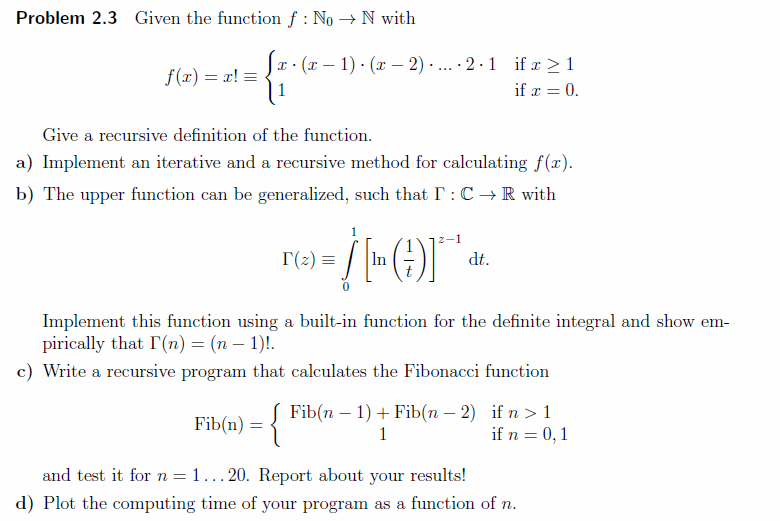
\includegraphics[width=1\textwidth]{chapters/images/desc-2-3}
\end{figure}


\subsubsection{a)}

\begin{lstlisting}[caption=Problem 2.3 a)]
n = int(input("n = "));

factorialIterative = 1;

for i in range(n):
    factorialIterative *= (i + 1);

print("iterative result: " + str(factorialIterative));

def factorialFunc(x):
    if x <= 0: return 1;
	
    return x * factorialFunc(x - 1);

factorialRecursive = factorialFunc(n);

print("recursive result: " + str(factorialRecursive));
\end{lstlisting}

The results of both factorial functions are:

\begin{lstlisting}[caption=Result of 2.3 a), keywordstyle=\color{black}]
n = 9
iterative result: 362880
recursive result: 362880
\end{lstlisting}


\subsubsection{b)}

The integral can be calculated with a built-in function from the scipy library.

\begin{lstlisting}[caption=Problem 2.3 b)]
import scipy.integrate as itg;

def bFunc(t, z):
	return math.pow(math.log(1 / t), z - 1);

for i in range(1, 7):
	factorialResult = factorialFunc(i - 1);
	integrateResult = itg.quad(lambda x: bFunc(x, i), 0, 1);
	
	print("n = " + str(i));
	print("(n - 1)! = " + str(factorialResult));
	print("Gamma(n) = " + str(integrateResult));
\end{lstlisting}

The results are:

\begin{lstlisting}[caption=Result of 2.3 b), keywordstyle=\color{black}]
n = 1
(n - 1)! = 1
Gamma(n) = (1.0, 1.1102230246251565e-14)

n = 2
(n - 1)! = 1
Gamma(n) = (1.0000000000000004, 1.6653345369377348e-15)

n = 3
(n - 1)! = 2
Gamma(n) = (2.0000000000000018, 1.687538997430238e-14)

n = 4
(n - 1)! = 6
Gamma(n) = (6.000000000000022, 2.9398705692074145e-13)

n = 5
(n - 1)! = 24
Gamma(n) = (24.00000000000007, 3.4425795547576854e-12)

n = 6
(n - 1)! = 120
Gamma(n) = (120.00000000002257, 2.0904167286062147e-10)
\end{lstlisting}

The values of the gamma function are not exact because the quad function only calculates an approximation. The second value that's returned is an estimation of the error.

\subsubsection{c)}

\begin{lstlisting}[caption=Problem 2.3 c)]
def fibonacciFunc(x):
	if x <= 1: return 1;
	
	return fibonacciFunc(x - 1) + fibonacciFunc(x - 2);

for i in range(1, 21):
	fib = fibonacciFunc(i);
	print("fib(" + str(i) + ") = " + str(fib));
\end{lstlisting}

The calculated elements of the Fibonacci sequence are:

\begin{lstlisting}[caption=Result of 2.3 c), keywordstyle=\color{black}]
fib(1) = 1
fib(2) = 2
fib(3) = 3
fib(4) = 5
fib(5) = 8
fib(6) = 13
fib(7) = 21
fib(8) = 34
fib(9) = 55
fib(10) = 89
fib(11) = 144
fib(12) = 233
fib(13) = 377
fib(14) = 610
fib(15) = 987
fib(16) = 1597
fib(17) = 2584
fib(18) = 4181
fib(19) = 6765
fib(20) = 10946
\end{lstlisting}

As it can be seen, the Fibonacci function seems to grow exponentially.


\subsubsection{d)}

\begin{lstlisting}[caption=Problem 2.3 d)]
runtimes = [];

for i in range(30):
	timeStart = time.time();
	fibonacciFunc(i);
	ms = 1000 * (time.time() - timeStart);
	runtimes.append(ms);

plt.plot(runtimes);
plt.xlabel('x');
plt.ylabel('runtime fib(x) [ms]');
plt.show();
\end{lstlisting}

The graph of the runtime of the Fibonacci sequence looks like this:

\begin{figure}[!ht]
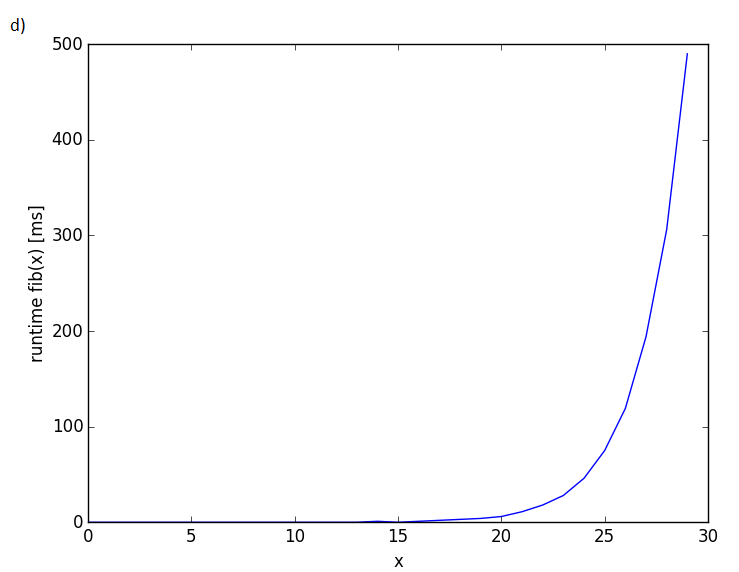
\includegraphics[width=1\textwidth]{chapters/images/figure-2-3-d}
\caption{Runtime of the Fibonacci function}
\end{figure}

As well as the $y$ values of the Fibonacci function, its runtime seems to grow exponentially too.


\subsection{Problem 2.4}

%\begin{figure}[!ht]
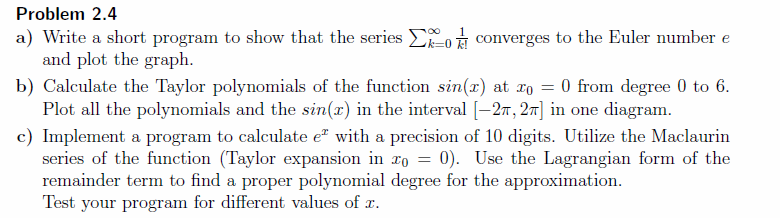
\includegraphics[width=1\textwidth]{chapters/images/desc-2-4}
%\end{figure}


\subsubsection{a)}

To graphically show that the series converges to the Euler number $e$, the series could be defined as a function $f(x)$ where $x$ defines the number of iterations of the sum, like $f(x) = \sum_{k = 0}^{\lfloor x \rfloor} \frac{1}{k!}$.

\begin{lstlisting}[caption=Problem 2.4 a)]
def factorialFunc(x):
    if x <= 0: return 1;
	
    return x * factorialFunc(x - 1);

def aFunc(x):
	sum = 0
	for i in range(x):
		sum += (1.0 / factorialFunc(i));
	return sum;

results = [];
eulers = [];

for i in range(10):
	results.append(aFunc(i));
	eulers.append(math.e);

plt.plot(results);
plt.plot(eulers);
plt.xlabel('x');
plt.ylabel('y');
plt.show();
\end{lstlisting}

The graph of the function with a line for $e$ looks like this:

\newpage

\begin{figure}[!ht]
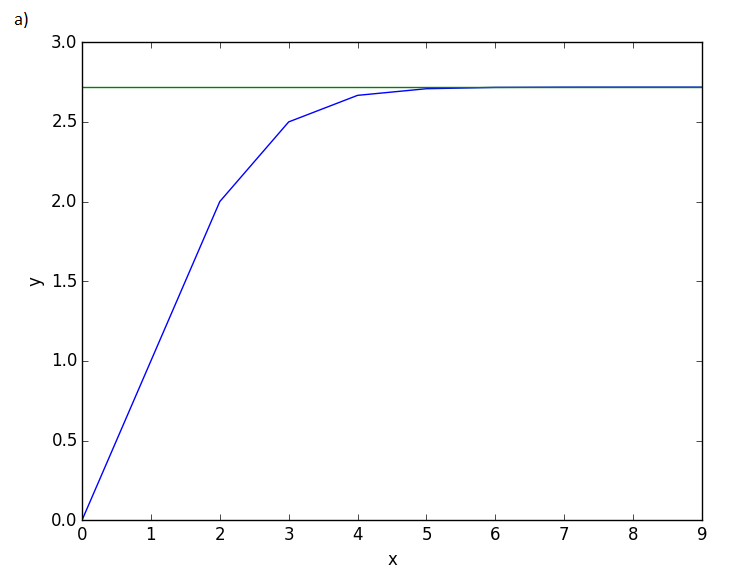
\includegraphics[width=1\textwidth]{chapters/images/figure-2-4-a}
\caption{Graphs of both functions}
\end{figure}

As it can be seen, after $x = 5$ there's hardly any difference visible in the graph.


\subsubsection{b)}

\begin{lstlisting}[caption=Problem 2.4 b)]
def bFunc(degree, x):
	sum = x;
	
	if (degree >= 3): sum -= (1.0 / 6.0) * pow(x, 3);
	if (degree >= 5): sum += (1.0 / 120.0) * pow(x, 5);
	
	return sum;

def bFunc2(degree):
	nSteps = 40;
	xStep = 4 * math.pi / (nSteps - 1);
	x = math.pi * -2;
	
	xses = [];
	results = [];
	
	for i in range(nSteps):
		xses.append(x);
		results.append(bFunc(degree, x));
		x += xStep;
	
	return [xses, results];

for i in range(0, 7):
	taylorFunc = bFunc2(i);
	plt.plot(taylorFunc[0], taylorFunc[1]);

plt.xlabel('x');
plt.ylabel('y');
plt.show();
\end{lstlisting}


The graph of the polynomials looks like the following:

\begin{figure}[!ht]
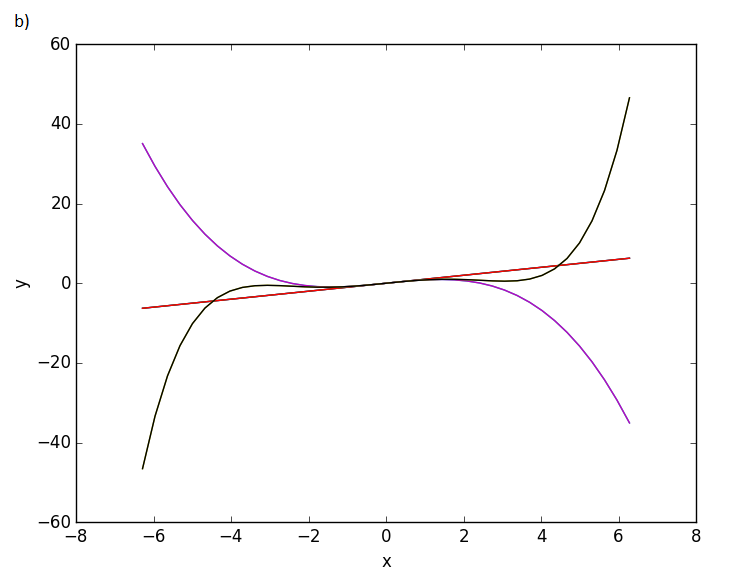
\includegraphics[width=1\textwidth]{chapters/images/figure-2-4-b}
\caption{Graphs of all Taylor series}
\end{figure}

Since $sin^{(2n)}(0) = 0$ for $n \in \mathbb{N}$, the respective term won't show up in the Taylor polynomial. Therefore, the Taylor polynomial for degree $(2n - 1)$ is the same as for degree $(2n)$ (with $n \in \mathbb{N}$). Because of that, only three different polynomials can be seen in the graph.

\subsubsection{c)}

\begin{lstlisting}[caption=Problem 2.4 c)]
ef eulerFunc(d, x):
	if (d <= 0): return 1;

	sum = 1;
	
	for i in range(1, d + 1):
		sum += pow(x, i) / (factorialFunc(i) + 0.0);
	
	return sum;

def getRemainder(n, x):
	xabs = abs(x);
	
	return (math.exp(xabs) * pow(xabs, n + 1)) / float(factorialFunc(n + 1));

def getDegree(x):
	n = 0;
	
	while n < 100:
		remainder = getRemainder(n, x);
		
		if (remainder < 1e-11): return n;
		
		n = n + 1;
		
	return -1;

for x in range(1, 6):
	deg = getDegree(x);
	eul = eulerFunc(deg, x);
	
	print("x = " + str(x) + " | degree = " + str(deg) + " | e(" + str(x) + ") = " + str(eul));
\end{lstlisting}


The resulting approximations as well as the necessary degree for the approximation to be as precise as wanted are the following:

\begin{lstlisting}[caption=Result of 2.4 c), keywordstyle=\color{black}]
x = 1 | degree = 14 | e(1) = 2.71828182846
x = 2 | degree = 19 | e(2) = 7.38905609893
x = 3 | degree = 23 | e(3) = 20.0855369232
x = 4 | degree = 28 | e(4) = 54.5981500331
x = 5 | degree = 32 | e(5) = 148.413159103
\end{lstlisting}

As it can be seen, with every step of $x$ the necessary degree has to increase by about 5.


\subsection{Problem 2.5}

\begin{figure}[!ht]
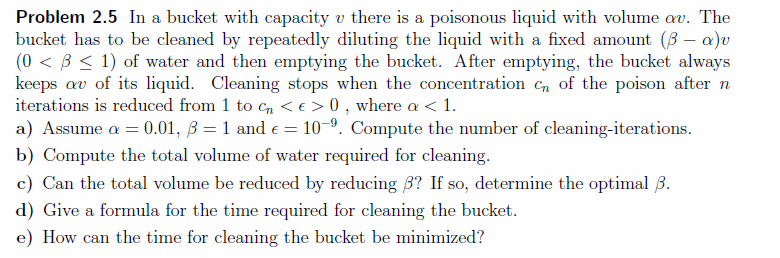
\includegraphics[width=1\textwidth]{chapters/images/desc-2-5}
\end{figure}


\subsubsection{a)}

With each cleaning iteration the concentration is multiplied by $\frac{\alpha}{\alpha + (\beta - \alpha)}$, which can be simplified to $\frac{\alpha}{\beta}$. The bucket can be defined as a class, with $\alpha$, $\beta$ and $\epsilon$ as attributes and the cleaning algorithm as function:

\begin{lstlisting}[caption=Problem 2.5 a)]
class Bucket:
	poison = 1;
	cleaningIterations = 0;
	waterUsed = 0;
	
	def __init__(self, alpha, beta, eps):
		self.alpha = alpha;
		self.beta = beta;
		self.eps = eps;
	
	def doOneClean(self):
		water = self.beta - self.alpha;
		self.waterUsed += water;
		
		self.poison = (self.alpha / float(self.beta)) * self.poison;
	
	def clean(self):
		while (self.poison >= self.eps):
			self.cleaningIterations += 1;
			self.doOneClean();

bu = Bucket(0.01, 1, 10e-9);
bu.clean();
\end{lstlisting}

The result is the following:

\begin{lstlisting}[caption=Result of 2.5 a), keywordstyle=\color{black}]
number of iterations: 5
\end{lstlisting}


\subsubsection{b)}

The necessary adjustments to the class are already in the code fragment of the subtask a) (lines 4 and 13). The result of the calculation is:

\begin{lstlisting}[caption=Result of 2.5 b), keywordstyle=\color{black}]
water used: 4.95 * v
\end{lstlisting}


\subsubsection{c)}

To calculate how much water is needed to reduce the poison to the required concentration, first a formula to calculate the number of required iterations is needed.
The concentration after $n$ iterations is $(\frac{\alpha}{\beta})^n$, which means the number of iterations to reach the required concentration $\epsilon$ is $\lceil log_{\frac{\alpha}{\beta}}(\epsilon) \rceil$.

The amount of water which is used per iteration is $(\beta - \alpha) * v$. Therefore, the amount of water required is $\lceil log_{\frac{\alpha}{\beta}}(\epsilon) \rceil * (\beta - \alpha) * v$.

To find out the optimal $\beta$ with $\alpha = 0.01$ and $\epsilon = 10^{-9}$, the calculation for the water that is needed can be defined as a function $f(\beta) = \lceil log_{\frac{0.01}{\beta}}(10^{-9}) \rceil * (\beta - 0.01)$ with $\beta \in (0, 1]$. Looking at the graph of this function shows that the lowest $y$ value is approaching 0, however the exercise description stated that the water is dilluted with $((\beta - \alpha) * v)$ of water, so the value of $\beta$ has to be greater than $\alpha$. Therefore the optimal $\beta$ in terms of water needed is the lowest possible value that is greater than $\alpha$.


\subsubsection{d)}

As already discovered in the previous subtask, the algorithm to determine the number of iterations is $\lceil log_{\frac{\alpha}{\beta}}(\epsilon) \rceil$. The cleaning time is the result of this calculation times the amount time required for one iteration.

\subsubsection{e)}

The number of iterations, which is proportional to the cleaning time, get smaller the smaller $\frac{\alpha}{\beta}$ is. Therefore, with $\alpha$ as small and $\beta$ as big as possible the time for cleaning the bucket can be minimized. Assuming that $\alpha$ can't be adjusted the best possible value for $\beta$ would be 1.

